\chapter{Discussion}
\label{chp:discussion}

In this chapter, the results from the formal analysis will be evaluated and compared. If an attack were discovered in the analysis, possible improvements and alternatives will be suggested.


\section{Evaluation of Authentication Properties}


Table \ref{tab:scyther-results-auth} shows the security properties related to authentication for the three protocols that have been verified by Scyther. In the section for entity authentication, we assume that successful verification of the weakest property in the hierarchy of authentication properties, Aliveness, is enough to earn a checkmark in the column. However, Aliveness has to hold for the role in the claims of all the other roles, meaning that all roles that claim aliveness for role $A$ has to be successfully verified to obtain the check mark. In cases where the property is not applicable, for instance claiming entity authentication for role $C$ in \gls{apkes} or \gls{akes}, a dash is inserted. The authentication phase in \gls{sakes} only includes $A$, $B$, and $C$, while the key establishment phase includes the claim for entity authentication of role $D$.

\begin{table}[h]
\centering
\resizebox{\textwidth}{!}{%
\begin{tabular}{lccccccccccccc}\hline
\multicolumn{1}{p{1cm}}{Protocol}
& \multicolumn{4}{p{4cm}}{Entity authentication}
& \multicolumn{4}{p{4cm}}{Implicit key\newline authentication}
& \multicolumn{4}{p{5cm}}{Explicit key authentication}\\
 & Of A & Of B & Of C & Of D & Of A & Of B & Of C & Of D & Of A & Of B & Of C & Of D\\ \hline
APKES & \checkmark & \checkmark & $-$ & $-$ & \checkmark & \checkmark & $-$ & $-$ & $\times$ & \checkmark & $-$ & $-$\\
AKES & \checkmark & \checkmark & $-$ & $-$ & \checkmark & \checkmark & $-$ & $-$ & \checkmark & \checkmark & $-$ & $-$\\
SAKES & \checkmark & \checkmark & \checkmark & \checkmark & \checkmark & \checkmark & $-$ & \checkmark & $\times$ & $\times$ & $-$ & $\times$ \\ \hline
\end{tabular}}
\caption{Table of the security properties for authentication that are satisfied in the different protocols.}
\label{tab:scyther-results-auth}
\end{table}

\gls{apkes} is only able to achieve explicit key authentication for the responding role $B$ because the \texttt{HELLOACK} that is sent from $B$ to $A$ is authenticated by using the shared secret from the pluggable scheme. \gls{akes} fixes this by computing the session key before sending the \texttt{HELLOACK} and use the session key to compute the \gls{mac-auth}. Hence it achieves explicit key authentication. As for \gls{sakes}, the session key can not be computed without the other side of the key establishment sending its secret key to the power of the generator. There is not, however, any message passing proving that the session key is in fact computed, and therefore, no explicit key authentication is provided by either party, which means that during its key establishment process, \gls{sakes} is only able to provide implicit key authentication. $A$ is included in this process even though it is not directly computing the key, but receives it from the router $B$.

\section{Evaluation of Key Secrecy Properties}

Table \ref{tab:scyther-results-sec} shows the results related to the secrecy of the computed keys in the various schemes. In all three schemes, the computed key is verified to be secret, which is the most valuable property in key establishment schemes. Key control is not directly modelled and verified, but can verified manually by confirming that each side in the key establishment phase has to contribute to the computation of the key. Known-key security is modelled by allowing the adversary to obtain session keys from other sessions than the current one. The importance of verifying this property is so that there is not possible to compute future session keys from knowledge of previous ones. \gls{akes} holds for this property, as well as \gls{sakes}, while \gls{apkes} does not claim this property as it computes a long-term pairwise key rather than session keys.

\begin{table}[h]
\centering
\resizebox{\textwidth}{!}{%
\begin{tabular}{lccccc}\hline
\multicolumn{1}{p{1cm}}{Protocol}
& \multicolumn{1}{p{2cm}}{Secrecy of\newline key}
& \multicolumn{1}{p{2cm}}{Key control}
& \multicolumn{1}{p{3cm}}{Known-key security}
& \multicolumn{1}{p{3cm}}{Forward Secrecy}
& \multicolumn{1}{p{3cm}}{Key compromise\newline impersonation}\\
 \hline
APKES & \checkmark & \checkmark & $-$ & $-$ & $-$ \\
AKES & \checkmark & \checkmark & \checkmark & $-$ & $-$ \\
SAKES & \checkmark & \checkmark & \checkmark & $\times$ & $\times$ \\ \hline
\end{tabular}}
\caption{Table of the security properties for secrecy that are satisfied in the different protocols.}
\label{tab:scyther-results-sec}
\end{table}

As explained in Section \ref{sec:attributes}, forward secrecy is a property where the compromise of the long-term key used to generate session keys does not lead to compromise of previous sessions. The Diffie-Hellman key agreement is one of the most well-known schemes that provide forward secrecy. \gls{sakes} leverage this type of agreement, and therefore it should provide forward \gls{pfs} or at least \gls{wpfs}.

When looking at Table \ref{tab:scyther-results-sec}, this is not the case based on the models that this thesis presents. If we observe the protocol more closely, we see that the server has, in fact, a fixed public key pair $(Pk_D, Sk_D)$, and do not generate anything fresh for each session. This means that if the key pair of the remote server is compromised, all previous sessions would be compromised as well, given that the adversary has recorded the messages passed in previous session key establishments. \gls{akes} generates session keys as well, but as these keys are computed using a symmetric key, it is infeasible for the protocol to achieve forward secrecy. Forward secrecy is not, however, a claimed secrecy property of either \gls{apkes} nor \gls{akes}.


\section{Comparison}

\subsubsection{APKES versus AKES}

Both infrastructures focus on device-to-device communication without any in-between routers to forward messages. \gls{akes} is merely an improvement over \gls{apkes}, which addresses its known issues. From the results in Table \ref{tab:scyther-results-auth} and Table \ref{tab:scyther-results-sec}, we see that the security properties provided in both protocols are almost identical, but as we know: \gls{akes} generates session keys. The advantage with \gls{akes} is its support for mobility in terms of handling reboot of nodes and deleting disappeared neighbours to save precious storage space on devices that these protocols target.

Also, \gls{akes} uses its derived session key to authenticate the message providing the initiating party with its nonce, which eventually ends in the protocol achieving explicit key authentication. Overall, \gls{akes} is naturally the best choice of the two based on its security properties and built-in mechanisms which gives it more robustness when deployed in a dynamic \gls{6lowpan} network.

\subsection{AKES versus SAKES}

Both \gls{akes} and \gls{sakes} are protocols for establishing session keys in \gls{6lowpan} networks, but the infrastructure for the following protocol includes both \gls{6lowpan} routers and border routers, as well as a remote server which the devices connect to. Based on the security properties in Table \ref{tab:scyther-results-auth} and Table \ref{tab:scyther-results-sec}, we see that both protocols provide the same security properties. However, based on the Scyther analysis presented in Section \ref{sec:akes-analysis} and Section \ref{sec:sakes-analysis}, \gls{akes} seems to be the protocol that is most carefully designed. Multiple attacks are introduced that target different phases of \gls{sakes}, which may indicate that the suggested protocol is not a preferable protocol to use for key establishment in your next \gls{6lowpan} network.

Apart from the attacks discovered in the analysis, \gls{sakes} have a more thorough authentication hierarchy, where the trusted authentication module provides authentication of each device and router in the network for each session key establishment. Authentication in \gls{akes} is solely based on that if the node is capable of establishing keys using the shared secret, it is authenticated.

It is difficult to recommend \gls{sakes} over \gls{akes} as a protocol to use in \gls{6lowpan} as it is wrong in its original proposed form, and since its complexity leads to a security analysis where the model had to be split into separate phases. Also, as they are proposed for different infrastructures. However, \gls{akes} can successfully establish session keys for device-to-device communication, and is also implemented and tested in the Contiki operating system \cite{krentz2015handling}.

%\gls{akes} is merely an improvement of \gls{apkes} and addresses the issues that was originally discovered in \gls{apkes}. While relying on the same three-way handshake and the use of pluggable scheme, \gls{akes} introduces more parameters for handling mobility, as well as additional protocols for discovering and deleting nodes at runtime. Table \ref{tab:scyther-results-auth} shows that \gls{akes} achieves a stronger notion of key authentication over \gls{apkes}, namely explicit key authentication for both parties. The main difference between these two schemes is the keys that are generated. \gls{akes} generates a fresh session key, while \gls{apkes} generates a pairwise, long-term key. The advantages with \gls{akes} is that using a session key solves multiple of the weaknesses with \gls{apkes}, especially those related to mobility and deadlocks that occurs on reboots.


%\gls{sakes} consists of more infrastructure than what \gls{akes} and \gls{sakes} have described, which makes the key establishment process more complicated. As seen in the analysis presented in Section \ref{sec:anal-sakes}, \gls{sakes} has a broad set of possible protocol traces. Partially because of bad protocol design, and partially because of the amount of entities and message passing that has to be done to compute and distribute the session key.


%\subsection{Use cases}

% More on use cases / comparison?

%\gls{akes} and \gls{apkes} describe communication between low-power devices without any centralized routers or authentication modules, and no remote server that provides services to network compared to \gls{sakes}. This makes \gls{akes} and \gls{apkes} a more suitable option for systems that have special requirements to low-power infrastructure, and which are not able to provide more powerful devices to act as routers and border routers. Also, as \gls{akes} and \gls{apkes} is targeted on device-to-device communication, it enables the network to act more as a unit that exchanges information across devices. Seen in connection with the scenario presented in Section \ref{sec:iot}, these protocols would enable the garage door and car to communicate directly with each other. \gls{akes} was successfully verified for an unbounded state space in Section \ref{sec:akes-analysis}, which may indicate that it is an applicable scheme for \gls{6lowpan} networks that target communication directly between the devices.

%\gls{sakes}, as it is suggested, allows for devices to connect directly to the remote server, but there are no specifications on how to provide device-to-device communication, which means that communication between the two doors has to go through the remote server. \gls{sakes}, if implemented correctly and efficiently could be used in larger systems where each end device have a certain task, and only needs to communicate its sensor data to the remote server. Examples of such networks could be smart grids which sends data to the control center, where the control center proceeds to instruct the sensors on what to do next.



\section{Suggested Improvements}

Flaws for both \gls{apkes} and \gls{sakes} have been discovered in the formal analysis presented in this thesis. This section aims to propose possible improvements to the protocols that could fix or improve the protocol.

\subsection{Possible Improvements for APKES}

\subsubsection{Use the pairwise session key to authenticate the HELLOACK}

\gls{apkes} does provide verifiable and secure key establishment. One improvement, however, could be to use the pairwise session key to authenticate the \texttt{HELLOACK} that is sent between $B$ and $A$ in Figure \ref{fig:apkes-handshake}, instead of the shared secret. By doing so, the scheme would achieve explicit key authentication of $B$ to $A$ as well, and behave much like \gls{akes} while still generating a pairwise symmetric key.


%\subsection{AKES}

\subsection{Possible Improvements for SAKES}
\label{subsec:sakes-fix}

\subsubsection{Achieve authentication in the authentication phase by returning nonces}


As presented in Section \ref{subsec:sakes-auth}, certain authentication claims fail in \gls{sakes}. Two of them are \texttt{Weakagree} claims in role $A$ for the router $B$ and the border router $C$. These can be fixed by adding the nonce $N_A$, which was initially generated by the end device to the response that is sent from the border router to the end device for confirming the identity of the router $B$. Listing \ref{lst:fix-weakagree-auth} shows how this is implemented in the improved model of \gls{sakes}, which can be found in Appendix \ref{app:sakes-fixed-auth}.\\

\newpage

\begin{lstlisting}[caption={Fix to the SAKES protocol to provide weak agreement for the end device in the authentication phase.}, label={lst:fix-weakagree-auth}]
	# Previous:
	send_6(C, A, B, Nc, MAC(B, Nc, k(A, C)); # In role C
	recv_6(C, A, B, Nc, MAC(B, Nc, k(A, C)); # In role A
	
	# Fix:
	send_6(C, A, B, Na, Nc, MAC(B, Na, Nc, k(A, C)); # In role C
	recv_6(C, A, B, Na, Nc, MAC(B, Na, Nc, k(A, C)); # In role A
\end{lstlisting}

The next step is to acheive non-injective synchronization and data agreement for the authentication phase. As discovered in the attacks from Section \ref{subsec:sakes-auth}, the issue lies in two messages. The first message is the request that is created at the end device and sent to the router. To avoid that the request can be reused in pair with an unrelated nonce $N_{B2}$ from another session, we have to add the received nonce $N_{B1}$ in the initial request as seen in Listing \ref{lst:fix-nisynch-ac-auth}. By adding this nonce, the protocol achieves both non-injective synchronization and data agreement for the end device $A$ and the border router $C$.\\

\begin{lstlisting}[caption={Fix to the SAKES protocol to provide non-injective synchronization and data agreement for the end device and the border router during the authentication phase.}, label={lst:fix-nisynch-ac-auth}]
	# Previous
	send_3(A, B, {A, B, D}k(A,C), A, Na, MAC); # In role A
	recv_3(A, B, {A, B, D}k(A,C), A, Na, MAC); # In role B

	# Fix
	send_3(A, B, {A, B, D}k(A,C), A, Na, Nb, MAC); # In Role A
	recv_3(A, B, {A, B, D}k(A,C), A, Na, Nb, MAC); # In Role B
\end{lstlisting}


Lastly, the protocol lacks non-injective synchronization and data agreement for the router $B$. When the router relays the request from the end device to the border router, it receives a signed proof of identities and an ephemeral public key pair from the border router. There is not, however, confirmation of that this is the intended response to that particular request. It may be possible that the returned identities and key pair are actually from a different session, hence the protocol is not able to fulfil the two claims non-injective synchronization and data agreement for the router $B$. If the border router $C$ is instructed to return the nonce $N_B$ that was generated by the router and sent with the request, the router can verify that the response corresponds to the initial request, and not a different session. Listing \ref{lst:fix-nisynch-b-auth} shows how this improvement can be added to the message.\\

\begin{lstlisting}[caption={Fix to the SAKES protocol to provide non-injective synchronization and data agreement for the router $B$ during the authentication phase.}, label={lst:fix-nisynch-b-auth}]
	# Previous
	send_5(C, B, {Signed-Proof, Pk, Sk, Nc}k(B, C)); # In role C
	recv_5(C, B, {Signed-Proof, Pk, Sk, Nc}k(B, C)); # In role B
	
	# Fix
	send_5(C, B, {Signed-Proof, Pk, Sk, Nb, Nc}k(B, C)); # In role C
	recv_5(C, B, {Signed-Proof, Pk, Sk, Nb, Nc}k(B, C)); # In role B
\end{lstlisting}
\newpage

\begin{figure}[H]
	\centering
	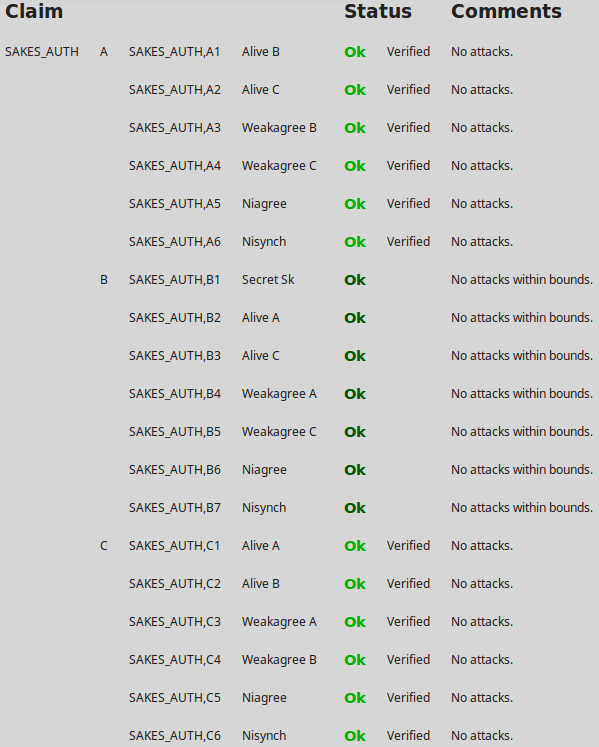
\includegraphics[scale=0.80]{analysis/sakes-fix-auth-verified.png}
	\caption{Result of verifying the fixed version of SAKES' authentication claims using Scyther.}
	\label{fig:sakes-fix-verified-auth}
\end{figure}

\subsubsection{Add nonces in the key establishment phase to remove malicious behaviour}

Above, the adding of nonces in the authentication phase was suggested to improve the level of authentication and protect the protocol against misbehaviour. This idea should also be transferred to the key establishment phase. When inspecting the protocol specification for \gls{sakes}, which can be reviewed in Figure \ref{fig:sakes-keys}, we observe that the nonce $N_A$, which the end device creates for each session request, is not returned to the end device along with the session key.

The formal security analysis of \gls{sakes} in Section \ref{sec:sakes-analysis} revealed attacks on the authentication of the end device during the key establishment, which can be reviewed in Figure \ref{fig:sakes-verified-keys-ab}. When inspecting the protocol, we observe that the protocol lacks the same type of message linking as explained above. More specific, the nonce that is generated by the end device at the start-up of the protocol, $N_B$, is not returned along with the session key.


\begin{lstlisting}[caption={Fix to the SAKES protocol to provide non-injective synchronization and data agreement for the end device $A$ during the key distribution.}, label={lst:fix-nisynch-a-keys}]
	# Previous
	send_3(B, A, {Nb, SessionKeyA}k(A, B)); # In role B
	recv_3(B, A, {Nb, SessionKeyA}k(A, B)); # In role A
	
	# Fix
	send_3(B, A, {Na, Nb, SessionKeyA}k(A, B)); # In role B
	recv_3(B, A, {Na, Nb, SessionKeyA}k(A, B)); # In role A
\end{lstlisting}

Not returning the $N_A$ nonce along with the session key removes the mapping between the request and the session key, effectively meaning that the end device is unable to detect which session the received session key belongs to. By adding this nonce as seen in Listing \ref{lst:fix-nisynch-a-keys} above, the model presented in Appendix \ref{app:sakes-keys-ab} would achieve both non-injective synchronization and data agreement for the end device as seen in Figure \ref{fig:sakes-fix-verified-keys-a-nisynch}. 

However, the attack on the \texttt{weakagree} claim in $A$ is still present in Figure \ref{fig:sakes-fix-verified-keys-a-nisynch}, and can be seen in Figure \ref{fig:sakes-attack-keys-a-weakagree-b} in Appendix \ref{app:attacks}. The attack claims to fake the sending of the nonce $N_B$ from the router to the end device, which means that the protocol is unable to prove that 

In the subsection on improving the authentication phase that was discussed previously in this section, weak agreement was provided for all the end device, the router, and the border router. As the attack found in the model of the isolated interaction between the end device and the router targets a message that was sent in authentication phase of the protocol, it may be that the attack is a consequence of the separation of the two phases, and not a direct attack on the protocol itself.


\begin{figure}[H]
	\centering
	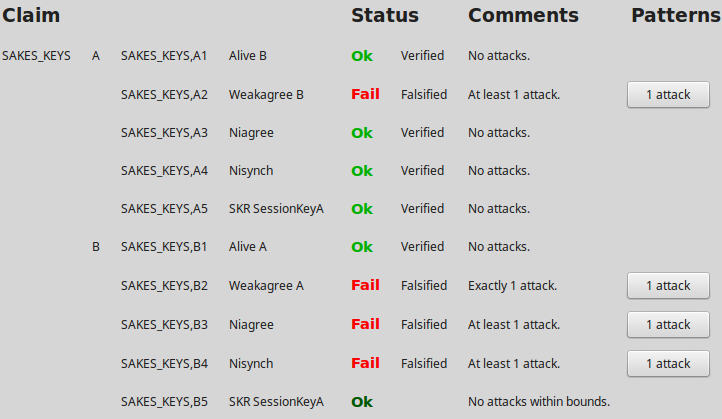
\includegraphics[scale=0.68]{analysis/sakes-keys-verified-a-nisynch-fix.png}
	\caption{Result of verifying the model of the key distribution in SAKES' using Scyther with a mapping between session and session key.}
	\label{fig:sakes-fix-verified-keys-a-nisynch}
\end{figure}



\subsubsection{Return the proof to the router to confirm the identity of the server}

In Section \ref{subsec:sakes-keys-results}, the results of Scyther's verification of the key establishment model was presented. As discussed, the two phases in \gls{sakes} has been divided into two separate models due to the large state-space. In the results, both claims for non-injective synchronization and data agreement for the router $B$ were falsified, in addition to the \texttt{weakagree} claim of the server $D$ in $B$'s claims. A theory was presented where these attacks were suggested to originate from the lack of mapping between the request to the server and its response, and also the absence of authentication of the server to the router.

To protect the protocol from an adversary that can forge the responses from the server, a suggestion was to include both the proof generated by the border router $C$ and the nonce $N_B$ in the response from the server, which can be done as seen in Listing \ref{lst:fix-nisynch-b-keys}.

\newpage

\begin{lstlisting}[caption={Fix to the SAKES protocol to provide authentication of the remote server D to the router B in the key establishment phase.}, label={lst:fix-nisynch-b-keys}]
	# Previous
	send_3(D, B, {Nd, g1(Sk(D), MAC}k(sk(D))); # In role D
	recv_3(D, B, {Nd, g1(Sk(D), MAC}k(sk(D))); # In role B

	# Fix
	send_3(D, B, {Nd, Nb, Signed-Proof, g1(Sk(D), MAC}k(sk(D))); # In role D
	recv_3(D, B, {Nd, Nb, Signed-Proof, g1(Sk(D), MAC}k(sk(D))); # In role B
\end{lstlisting}


\begin{figure}[H]
	\centering
	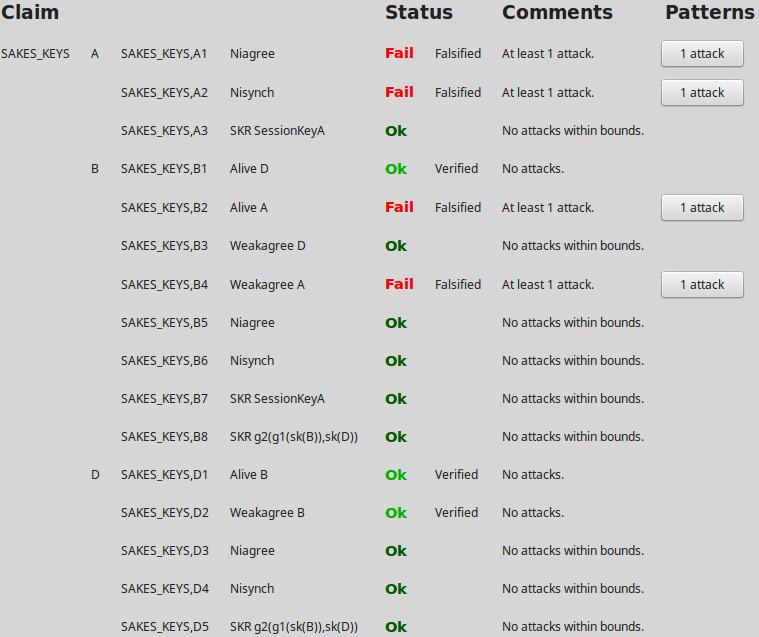
\includegraphics[scale=0.65]{analysis/sakes-keys-verified-proof-b.png}
	\caption{Result of verifying the model of the key distribution in SAKES' using Scyther where the server returns both the proof and the nonce $N_B$.}
	\label{fig:sakes-fix-verified-keys-b-proof}
\end{figure}

When running the model with the changes above in Scyther, the results in Figure \ref{fig:sakes-fix-verified-keys-b-proof} is returned. As we see, the protocol achieves both non-injective synchronization and data agreement, as well as weak agreement for the server $D$. We observe that the claims for non-injective synchronization and data agreement for $A$, as well as aliveness and weak agreement in $B$ are failing. However, these were previously addressed, where a possible solution were introduced and verified. When seeing these two results as one, all the claims in the protocol are essentially confirmed after the presented fixes.


\subsubsection{Use nonces instead of secret keys in the Diffie-Hellman key agreement}

\gls{sakes} uses the private key of an ephemeral key pair at the router side and the private of the server to generate the session key in a Diffie-Hellman manner. The reason for generating the key pair in the first place is to use them in the computation of the session key. Another usage is to sign the messages that are sent between the router and the server using the private key, and verify them with the public key. Generating public key pairs is a time consuming process for a server to do, especially if it has to do so for each session, and if the network of end devices that request services is large. Therefore, random nonces could be generated in addition to improve the security of the session keys that are generated in the key establishment phase. This approach will also allow for maintaining the signing capability of the server and the router.

Generating random nonces is relatively inexpensive compared to generating public key pairs. Let both $B$ and $D$ generate one nonce each, $N_{B2}$ and $N_{D2}$, to use in the key establishment phase. When $B$ sends its request to $D$, it also sends $g^{N_{B2}}$ to the server. At the server side, the server sends $g^{N_{D2}}$ in return to $B$, and computes the session key as $(g^{N_{B2}})^{N_{D2}}$. The advantage with this approach is that in the case of the server being compromised, the adversary would not be able to decrypt previous sessions since the nonces used to generate the session key are fresh at both sides each time. %The adversary may still use the signing key pair of $D$ to impersonate $D$ to the network and establish new sessions, but previous communication would be secure.


\subsubsection{Use Elliptic Curve Diffie-Hellman and the Elliptic Curve Digital Signature Algorithm}

Another suggestion is to use the \gls{ecdh} in conjunction with the \gls{ecdsa} \cite{johnson2001elliptic} in the key establishment phase. \gls{ecdh} uses \gls{ecc} public key pairs in the Diffie-Hellman key agreement. However, as the protocol generates an ephemeral public key pair for the router to use in each key establishment session, we need to handle authentication and integrity of the messages in addition. Authentication can be achieved by using the \gls{ecdsa} to sign the messages that are exchanged.

The protocol specifications of \gls{sakes} states that the key pair generated by the authentication module $C$ is an \gls{ecc} key pair, while no information is given about how the public key pair of the server $D$ is derived. As the server is assumed to be a computational powerful entity, it is fair to assume that it is capable of generating an \gls{ecc} public key pair as well.

As mentioned in Section \ref{sec:keyestablishment}, public-key cryptography is more computational expensive than symmetric cryptography, meaning that the energy consumption on the devices is significantly higher. However, given the architecture of \gls{sakes}, where more powerful routers utilizes public-key cryptography to generate the session key, it may be an feasible approach to use \gls{ecdh} and \gls{ecdsa} in the key establishment. 



%\begin{table}[h]
%\centering
%\resizebox{\textwidth}{!}{%
%\begin{tabular}{lcccccccccc}
%\multicolumn{1}{p{1.3cm}}{Protocol}
%& \multicolumn{4}{p{1.5cm}}{Entity\newline authentication}
%& \multicolumn{1}{p{2.2cm}}{Implicit key\newline authentication}
%& \multicolumn{4}{p{2.2cm}}{Explicit key\newline authentication}
%& \multicolumn{1}{p{2.6cm}}{Key compromise impersonation}
%& \multicolumn{1}{p{1.1cm}}{Forward\newline Secrecy}
%& \multicolumn{1}{p{1.75cm}}{Known-key\newline security}
%& \multicolumn{1}{p{1cm}}{Key\newline control}
%& \multicolumn{1}{p{1.0cm}}{Secrecy\newline of key}\\
% & Of A & Of B & Of C & Of D &  & Of A & Of B & Of C & Of D &  &  & &\\ \hline
% APKES & \checkmark & \checkmark & - & - & \checkmark & \checkmark & x & x & x & x & \checkmark & \checkmark & \checkmark\\
% AKES & \checkmark & \checkmark & - & - & \checkmark & \checkmark & \checkmark & x & x & \checkmark & \checkmark & \checkmark\\
% SAKES & x & - & - & x & x  & - & - & x & x & x & x & x & x & x\\ \hline
%\end{tabular}}
%\caption{Table of the security properties that are satisfied in the different protocols.}
%\label{tab:scyther-results}
%\end{table}